\documentclass[11pt,a4paper]{article}

\usepackage[a4paper,margin=1in]{geometry}
\usepackage{amsmath}
\usepackage{amssymb}
\usepackage{booktabs}
\usepackage{array}
\usepackage{longtable}
\usepackage{graphicx}
\usepackage{float}
\usepackage{placeins}
\usepackage{graphicx}
\usepackage{float}
\usepackage{placeins}
\usepackage{hyperref}
\usepackage{enumitem}
\usepackage{hyperref}
\usepackage{enumitem}
\usepackage{titlesec}
\usepackage{listings}
\usepackage{xcolor}

\hypersetup{
colorlinks=true,
linkcolor=blue,
urlcolor=blue
}

\lstset{
language=Python,
basicstyle=\ttfamily\small,
keywordstyle=\color{blue},
commentstyle=\color{green!50!black},
stringstyle=\color{red},
numbers=left,
numberstyle=\tiny,
stepnumber=1,
breaklines=true,
frame=single,
showstringspaces=false
}

\renewcommand{\arraystretch}{1.4}

\begin{document}
\raggedbottom

\setlength{\textfloatsep}{10pt}
\setlength{\floatsep}{8pt}
\setlength{\intextsep}{8pt}

\clubpenalty=10000
\widowpenalty=10000
\displaywidowpenalty=10000

\begin{center}

{\Large \textbf{Shiv Nadar University Chennai}}

\vspace{0.3cm}

\begin{tabular}{|p{4cm}|p{8cm}|p{2cm}|}
\hline
Degree \& Branch &
B.Tech Artificial Intelligence \& Data Science &
Semester V\\
\hline
Subject Code \& Name &
CS3807 -- Deep Learning Laboratory &
AY: 2026--27\\
\hline
\end{tabular}

\vspace{0.7cm}

{\Large \textbf{Experiment 3}}

\vspace{0.2cm}

{\large \textbf{Implementation of Convolutional Neural Networks (CNNs) for Image Classification}}

\end{center}

\section*{1. Objective}

The objective of this experiment is to understand the working principle of Convolutional Neural Networks (CNNs) by implementing the individual building blocks of a CNN -- the convolution operation, stride and padding, feature map visualization, max pooling and average pooling -- from first principles, and subsequently by constructing, training and evaluating a complete CNN in PyTorch for multi-class image classification on the CIFAR-10 dataset. The experiment further aims to programmatically verify the parameter count of every layer, to compare pooling strategies and kernel configurations empirically, and to analyse the trained network's performance using standard classification metrics such as Accuracy, Precision, Recall, F1-score, the Confusion Matrix and the Classification Report.

\section*{2. Learning Outcomes}

Students will be able to

\begin{enumerate}
\item Explain the convolution operation.
\item Compute output dimensions using stride and padding.
\item Visualize feature maps.
\item Implement max pooling and average pooling.
\item Calculate CNN parameters.
\item Build a CNN for image classification.
\item Evaluate CNN performance.
\end{enumerate}

\section*{3. Background Theory}

A Convolutional Neural Network (CNN) is a class of deep feedforward network specialized for processing data with a grid-like topology, such as images. Unlike the Multi-Layer Perceptron studied in Experiment 2, which treats every pixel as an independent, flattened input feature, a CNN preserves the spatial structure of the image and exploits local pixel correlations through a small, shared set of learnable filters. A typical CNN consists of the following building blocks.

\begin{itemize}
\item Convolution Layer
\item Activation Layer
\item Pooling Layer
\item Fully Connected (Dense) Layer
\end{itemize}

The convolution operation itself is defined as

\[
Y(i,j) = \sum_{m}\sum_{n} X(i+m,\,j+n)\,K(m,n)
\]

where $X$ is the input image, $K$ is the convolution kernel (filter) and $Y$ is the resulting feature map. Each kernel slides across the input image, computing an element-wise product with the underlying pixel values at every position and summing the result into a single output value, so that different kernels highlight different visual characteristics of the image such as edges, textures or smooth regions.

The spatial size of the resulting feature map depends on the input size, the kernel size, the padding and the stride, according to

\[
\left\lfloor\frac{N-F+2P}{S}\right\rfloor + 1
\]

where $N$ is the input size, $F$ is the filter (kernel) size, $P$ is the amount of zero-padding applied to each side of the input, and $S$ is the stride with which the kernel moves across the input. A larger kernel or a larger stride reduces the size of the resulting feature map, while padding can be used to control -- and in the ``same'' case, preserve -- the spatial dimensions of the output.

\subsection*{Pooling}

A pooling layer reduces the spatial dimensions of a feature map while retaining its most important information, thereby reducing computation in subsequent layers and providing a degree of translation invariance. Max pooling retains the maximum activation within every pooling window, which tends to preserve the strongest, most discriminative activations (edges and prominent shapes), whereas average pooling retains the mean activation within every window, which produces a smoother, more diffused output. For a $2\times2$ max pooling filter applied to the feature map

\[
\begin{bmatrix}
1 & 5 & 2 & 3\\
7 & 8 & 1 & 0\\
4 & 6 & 9 & 5\\
2 & 3 & 1 & 8
\end{bmatrix}
\rightarrow
\begin{bmatrix}
8 & 3\\
6 & 9
\end{bmatrix}
\]

each $2\times2$ window is replaced by its maximum value, halving both spatial dimensions of the input.

\subsection*{CNN Architecture}

The CNN implemented in this experiment follows the classical architecture

\begin{center}
Input $\rightarrow$ Conv $\rightarrow$ ReLU $\rightarrow$ MaxPool $\rightarrow$ Conv $\rightarrow$ ReLU $\rightarrow$ MaxPool $\rightarrow$ Flatten $\rightarrow$ Dense $\rightarrow$ Softmax
\end{center}

Each convolution layer is followed immediately by a Rectified Linear Unit (ReLU) activation, $f(z) = \max(0,z)$, which introduces the non-linearity required to learn complex visual patterns, and a max pooling layer, which progressively reduces the spatial resolution of the feature maps while increasing the number of channels. After the final pooling stage, the three-dimensional feature volume is flattened into a one-dimensional vector and passed through one or more fully connected (Dense) layers, culminating in an output layer of 10 neurons corresponding to the 10 CIFAR-10 classes. During training, the raw output scores (logits) of this final layer are converted into class probabilities using the Softmax function

\[
\hat{y}_i = \frac{e^{z_i}}{\displaystyle\sum_{j=1}^{10} e^{z_j}}, \qquad i = 1,2,\dots,10
\]

and the network is trained by minimizing the Cross-Entropy loss between the predicted probability distribution and the true class label, with the Adam optimizer used to update every weight and bias in the network via backpropagation.

\subsection*{Parameter Calculation}

The number of trainable parameters contributed by a convolution layer with $F\times F$ kernels, $C_{in}$ input channels and $C_{out}$ output filters is

\[
\left(F \times F \times C_{in} + 1\right) \times C_{out}
\]

where the additional $+1$ accounts for the bias term of every filter. For example, a convolution layer with 16 filters of size $3\times3$ operating on a $32\times32\times3$ RGB image requires

\[
(3\times3\times3+1)\times16 = (27+1)\times16 = 448
\]

trainable parameters. The number of parameters contributed by a fully connected (Dense) layer with $n_{in}$ input features and $n_{out}$ output neurons is simply $(n_{in}+1)\times n_{out}$. Since convolution layers reuse the same small kernel across every spatial location of the input, they require dramatically fewer parameters than a fully connected layer of comparable output size, which is one of the central architectural advantages of the CNN over the MLP for image data, and is verified programmatically in Section 8 of this report.

\section*{4. Dataset Description}

The experiment uses the \textbf{CIFAR-10 Dataset}, a widely used benchmark dataset in the computer vision community, consisting of small colour photographs of real-world objects and animals, downloaded automatically using \texttt{torchvision.datasets.CIFAR10}.

\vspace{0.3cm}

\begin{center}
\begin{tabular}{|p{5cm}|p{7cm}|}
\hline
\textbf{Property} & \textbf{Value}\\
\hline
Dataset Name & CIFAR-10\\
\hline
Source & \texttt{torchvision.datasets.CIFAR10}\\
\hline
Training Images & 50{,}000\\
\hline
Testing Images & 10{,}000\\
\hline
Image Size & $32 \times 32 \times 3$ (RGB)\\
\hline
Target Classes & 10\\
\hline
Missing Values & None\\
\hline
Learning Type & Supervised Learning\\
\hline
Problem Type & Multi-class Image Classification\\
\hline
\end{tabular}
\end{center}

\vspace{0.15cm}
\textbf{Target Classes}

\begin{center}
\begin{tabular}{|c|p{9cm}|}
\hline
\textbf{Class Label} & \textbf{Description}\\
\hline
0 & airplane\\
\hline
1 & automobile\\
\hline
2 & bird\\
\hline
3 & cat\\
\hline
4 & deer\\
\hline
5 & dog\\
\hline
6 & frog\\
\hline
7 & horse\\
\hline
8 & ship\\
\hline
9 & truck\\
\hline
\end{tabular}
\end{center}

\vspace{0.3cm}

The dataset contains no missing values, and every one of the ten classes is represented by exactly 5{,}000 training images, resulting in a perfectly balanced class distribution -- this was confirmed by the class distribution plot in Section 9. Each image is provided directly as a $32\times32\times3$ tensor, with pixel intensities scaled to the range $[0,1]$ by the \texttt{ToTensor} transform, and no flattening is required since the convolution layers of the CNN operate directly on the two-dimensional spatial structure of the image.

\section*{5. Experimental Procedure}

The experiment was carried out using Python and PyTorch in Google Colab, with automatic detection of the available compute device (CUDA GPU or CPU) and a fixed random seed for reproducibility.

\begin{center}
\begin{tabular}{|p{5cm}|p{7cm}|}
\hline
\textbf{Property} & \textbf{Value}\\
\hline
Device Used & CUDA (Tesla T4 GPU)\\
\hline
Random Seed & 42\\
\hline
Framework & PyTorch\\
\hline
\end{tabular}
\end{center}

\vspace{0.3cm}

\subsection*{Task 1: Dataset Exploration}

The CIFAR-10 dataset was loaded directly using \texttt{torchvision.datasets.CIFAR10}. Ten representative sample images were displayed along with their true class names, the dataset dimensions were printed, and the class distribution across the training set was plotted.

\subsection*{Task 2: Convolution Kernel Size Comparison}

A single convolution layer was applied to a sample image using kernels of size $3\times3$, $5\times5$ and $7\times7$, with stride 1 and no padding, and the resulting feature map dimensions were recorded and tabulated.

\subsection*{Task 3: Hyperparameter Study (Stride and Padding)}

The effect of stride (1 and 2) and padding type (``Valid'', i.e. no padding, and ``Same'', i.e. padding chosen to preserve spatial size) on the output feature map size was computed analytically using the standard convolution output-size formula and tabulated for a $32\times32$ input with a $3\times3$ kernel.

\subsection*{Task 4: Feature Map Visualization}

Eight feature maps produced by the first convolution layer of the CNN were visualized for a sample training image, in order to inspect the low-level visual patterns learned by the earliest layer of the network.

\subsection*{Task 5: Pooling Comparison}

Max pooling and average pooling, each with a $2\times2$ window and stride 2, were applied to the same convolutional feature map, and the resulting output sizes and qualitative observations were compared and tabulated.

\subsection*{Task 6: CNN Construction and Training}

The CNN architecture described in Section 3 was implemented in PyTorch, its layer-wise structure and parameter count were printed, and the network was trained using the Adam optimizer for 20 epochs with a batch size of 32, with 5{,}000 images from the training set held out for validation.

\subsection*{Task 7: Model Evaluation}

After training, the model was evaluated on the untouched testing set of 10{,}000 images. Accuracy, weighted Precision, weighted Recall, weighted F1-score, the per-class Classification Report and the Confusion Matrix were computed and analysed.

\section*{6. Model Architecture}

The CNN implemented for this experiment consists of two convolution blocks followed by two fully connected layers, as summarized below.

\begin{center}
\begin{tabular}{|p{5.5cm}|p{9.5cm}|}
\hline
\textbf{Layer} & \textbf{Configuration}\\
\hline
Conv1 & Conv2d(3 $\rightarrow$ 32, kernel = 3$\times$3, stride = 1, padding = 1)\\
\hline
ReLU1 & ReLU activation\\
\hline
MaxPool1 & MaxPool2d(kernel = 2, stride = 2)\\
\hline
Conv2 & Conv2d(32 $\rightarrow$ 64, kernel = 3$\times$3, stride = 1, padding = 1)\\
\hline
ReLU2 & ReLU activation\\
\hline
MaxPool2 & MaxPool2d(kernel = 2, stride = 2)\\
\hline
Flatten & Flatten to a 4{,}096-dimensional vector (64 $\times$ 8 $\times$ 8)\\
\hline
FC1 & Linear(4{,}096 $\rightarrow$ 128), ReLU\\
\hline
FC2 (Output) & Linear(128 $\rightarrow$ 10), Softmax (via Cross-Entropy loss)\\
\hline
\end{tabular}
\end{center}

\vspace{0.15cm}

The network was compiled with the Cross-Entropy loss function and trained using the Adam optimizer with a learning rate of 0.001. Each convolution layer uses ``same'' padding ($P=1$ for a $3\times3$ kernel), so the spatial resolution is only reduced by the two max pooling layers, taking the $32\times32$ input down to $16\times16$ after the first pooling stage and $8\times8$ after the second, at which point the volume is flattened to $64\times8\times8=4{,}096$ features before being passed to the Dense layers.

\section*{7. Convolution and Hyperparameter Study}

\subsection*{7.1 Kernel Size Comparison}

Applying a single convolution layer with 8 output channels to a $32\times32\times3$ sample image, with stride 1 and no padding, for kernel sizes of $3\times3$, $5\times5$ and $7\times7$ produced the following feature map sizes.

\begin{center}
\begin{tabular}{|c|c|c|c|}
\hline
\textbf{Kernel Size} & \textbf{Input Size} & \textbf{Output Size} & \textbf{Output Channels}\\
\hline
$3\times3$ & $32\times32$ & $30\times30$ & 8\\
\hline
$5\times5$ & $32\times32$ & $28\times28$ & 8\\
\hline
$7\times7$ & $32\times32$ & $26\times26$ & 8\\
\hline
\end{tabular}
\end{center}

\vspace{0.15cm}

As expected from the output-size formula, the feature map shrinks by exactly $F-1$ pixels along each spatial dimension when no padding is used, so the $7\times7$ kernel produces the smallest feature map of the three configurations, while the number of output channels remains unaffected by the kernel size, since it is determined solely by the number of filters used.

\subsection*{7.2 Stride and Padding Comparison}

The output feature map size was computed for a $32\times32$ input with a $3\times3$ kernel, for both available strides and both padding conventions.

\begin{center}
\begin{tabular}{|c|c|c|c|}
\hline
\textbf{Stride} & \textbf{Padding} & \textbf{P} & \textbf{Output Size}\\
\hline
1 & Valid & 0 & $30\times30$\\
\hline
1 & Same & 1 & $32\times32$\\
\hline
2 & Valid & 0 & $15\times15$\\
\hline
2 & Same & 1 & $16\times16$\\
\hline
\end{tabular}
\end{center}

\vspace{0.15cm}

Increasing the stride from 1 to 2 roughly halves the output spatial dimension in every case, since the kernel now moves across the input in larger steps and therefore visits fewer positions. ``Same'' padding of $P=1$ compensates for the border pixels lost during a $3\times3$, stride-1 convolution and exactly preserves the $32\times32$ input resolution, whereas ``Valid'' padding (no padding) always shrinks the feature map, confirming the relationship $\lfloor(N-F+2P)/S\rfloor+1$ derived in Section 3.
\newpage
\section*{8. Parameter Calculation}

The trainable parameters of every layer in the implemented CNN were calculated programmatically using the standard convolution and dense-layer parameter formulas and cross-checked against PyTorch's own \texttt{model.parameters()} count.

\begin{center}
\begin{tabular}{|p{5cm}|p{4cm}|p{4cm}|}
\hline
\textbf{Layer} & \textbf{Formula} & \textbf{Parameters}\\
\hline
Conv1 & $(3\times3\times3+1)\times32$ & 896\\
\hline
Conv2 & $(3\times3\times32+1)\times64$ & 18{,}496\\
\hline
FC1 & $(4{,}096+1)\times128$ & 524{,}416\\
\hline
FC2 & $(128+1)\times10$ & 1{,}290\\
\hline
\textbf{Total} & & \textbf{545{,}098}\\
\hline
\end{tabular}
\end{center}

\vspace{0.15cm}

The manually calculated total of 545{,}098 trainable parameters matched exactly with the count returned by \texttt{model.parameters()} in PyTorch, confirming the correctness of the architecture and the parameter formulas of Section 3. It is worth noting that the two convolution layers together account for only 19{,}392 parameters (3.6\% of the total), while the first fully connected layer alone accounts for 524{,}416 parameters (96.2\% of the total) -- a direct illustration of how weight sharing keeps convolution layers parameter-efficient, while the transition from a spatial feature map to a flattened Dense layer remains comparatively expensive.

\section*{9. Pooling Comparison}

Max pooling and average pooling, each using a $2\times2$ window with stride 2, were applied to the same $32\times32$ feature map produced by the first convolution layer of the trained CNN.

\begin{center}
\begin{tabular}{|p{3.5cm}|p{2.5cm}|p{2.5cm}|p{6cm}|}
\hline
\textbf{Pooling Type} & \textbf{Input Size} & \textbf{Output Size} & \textbf{Observation}\\
\hline
Max Pooling & $32\times32$ & $16\times16$ & Retains the sharpest activations, preserving edges and prominent features\\
\hline
Average Pooling & $32\times32$ & $16\times16$ & Smooths the activations, retaining background context but losing sharp detail\\
\hline
\end{tabular}
\end{center}

\vspace{0.15cm}

Both pooling strategies reduce the spatial resolution identically, from $32\times32$ to $16\times16$, since the output size depends only on the pooling window size and stride, and not on the pooling operation itself. Qualitatively, however, the two operations behave very differently on the underlying activations: as shown in Section 12.4, the isolated, high-intensity pixels present in the original feature map are preserved almost unchanged by max pooling, whereas average pooling blends each activation with its neighbouring (largely zero) values, visibly dampening its magnitude.
\newpage
\section*{10. Training}

The CNN was trained using the Adam optimizer with a learning rate of 0.001, the Cross-Entropy loss function, a batch size of 32 and 20 epochs, with 45{,}000 images used for training and 5{,}000 images held out for validation.

\begin{center}
\begin{tabular}{|p{6cm}|p{6cm}|}
\hline
\textbf{Parameter} & \textbf{Value}\\
\hline
Optimizer & Adam (lr = 0.001)\\
\hline
Loss Function & Cross-Entropy\\
\hline
Epochs & 20\\
\hline
Batch Size & 32\\
\hline
Training Samples & 45{,}000\\
\hline
Validation Samples & 5{,}000\\
\hline
Final Training Accuracy (Epoch 20) & 96.81\%\\
\hline
Final Training Loss (Epoch 20) & 0.0921\\
\hline
Final Validation Accuracy (Epoch 20) & 67.32\%\\
\hline
Final Validation Loss (Epoch 20) & 2.1749\\
\hline
Total Training Time & 224.15 seconds\\
\hline
\end{tabular}
\end{center}

\vspace{0.15cm}

The training accuracy increased almost monotonically across all 20 epochs, from 48.12\% in the first epoch to 96.81\% by the twentieth epoch, while the training loss fell steadily from 1.4378 to 0.0921. The validation accuracy, by contrast, rose quickly during the first seven epochs to a peak of around 70.7\% and then plateaued and gradually declined to 67.32\% by the final epoch, while the validation loss began rising sharply from around epoch 6 onward, reaching 2.1749 by epoch 20. This widening gap between the training and validation curves, discussed further in Section 12, is a clear indication that the network began overfitting the training data in the later epochs.

\section*{11. Experimental Results}

The trained CNN was evaluated on the held-out testing set of 10{,}000 previously unseen CIFAR-10 images.

\begin{center}
\begin{tabular}{|p{6cm}|c|}
\hline
\textbf{Metric} & \textbf{Value}\\
\hline
Test Accuracy & 68.01\%\\
\hline
Precision (weighted) & 68.21\%\\
\hline
Recall (weighted) & 68.01\%\\
\hline
F1-Score (weighted) & 67.88\%\\
\hline
\end{tabular}
\end{center}

\vspace{0.15cm}

\begin{center}
\begin{tabular}{|p{3cm}|c|c|c|c|}
\hline
\textbf{Class} & \textbf{Precision} & \textbf{Recall} & \textbf{F1-Score} & \textbf{Support}\\
\hline
airplane & 0.66 & 0.77 & 0.71 & 1{,}000\\
\hline
automobile & 0.74 & 0.83 & 0.78 & 1{,}000\\
\hline
bird & 0.65 & 0.53 & 0.58 & 1{,}000\\
\hline
cat & 0.48 & 0.48 & 0.48 & 1{,}000\\
\hline
deer & 0.70 & 0.57 & 0.63 & 1{,}000\\
\hline
dog & 0.54 & 0.62 & 0.58 & 1{,}000\\
\hline
frog & 0.74 & 0.75 & 0.74 & 1{,}000\\
\hline
horse & 0.78 & 0.70 & 0.73 & 1{,}000\\
\hline
ship & 0.79 & 0.81 & 0.80 & 1{,}000\\
\hline
truck & 0.76 & 0.74 & 0.75 & 1{,}000\\
\hline
\textbf{Weighted Avg} & \textbf{0.68} & \textbf{0.68} & \textbf{0.68} & \textbf{10{,}000}\\
\hline
\end{tabular}
\end{center}

\vspace{0.15cm}

The per-class classification report shows that ship (79\% precision, 81\% recall), automobile (74\% precision, 83\% recall) and frog (74\% precision, 75\% recall) were classified most reliably, since these categories tend to have relatively distinctive colours, backgrounds and silhouettes at $32\times32$ resolution. In sharp contrast, the cat class obtained the weakest performance of all ten classes (48\% precision, 48\% recall), and the dog class was also comparatively weak (54\% precision, 62\% recall); this pairing is not a coincidence, since cats and dogs share a broadly similar body shape, posture and background context, making them the most visually ambiguous pair of classes in the dataset at this resolution.

\section*{12. Plots and Interpretation}

\subsection*{12.1 Sample Images}

\begin{figure}[H]
\centering
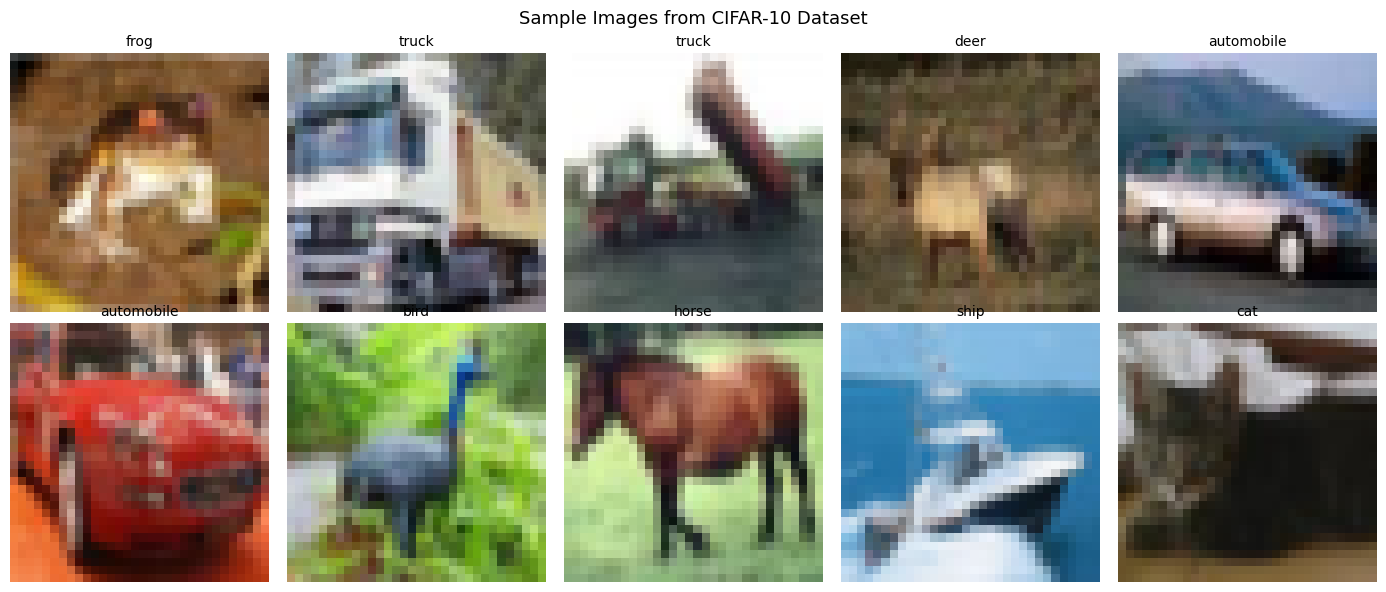
\includegraphics[width=0.95\textwidth]{plot1.png}
\caption{Ten Sample Images from the CIFAR-10 Dataset with True Class Labels}
\end{figure}

The sample images illustrate the visual diversity of the ten CIFAR-10 categories, spanning vehicles (automobile, truck, ship), animals (frog, deer, bird, horse, cat) and other objects, each photographed against varied, natural backgrounds. Several categories, such as ship and horse, are set against relatively uniform backgrounds (sky, sea, grass) that aid recognition, whereas classes such as cat and dog are frequently photographed at close range with cluttered backgrounds, foreshadowing the higher confusion observed between these two classes in Section 11.

\vspace{0.15cm}

\subsection*{12.2 Class Distribution}

\begin{figure}[H]
\centering
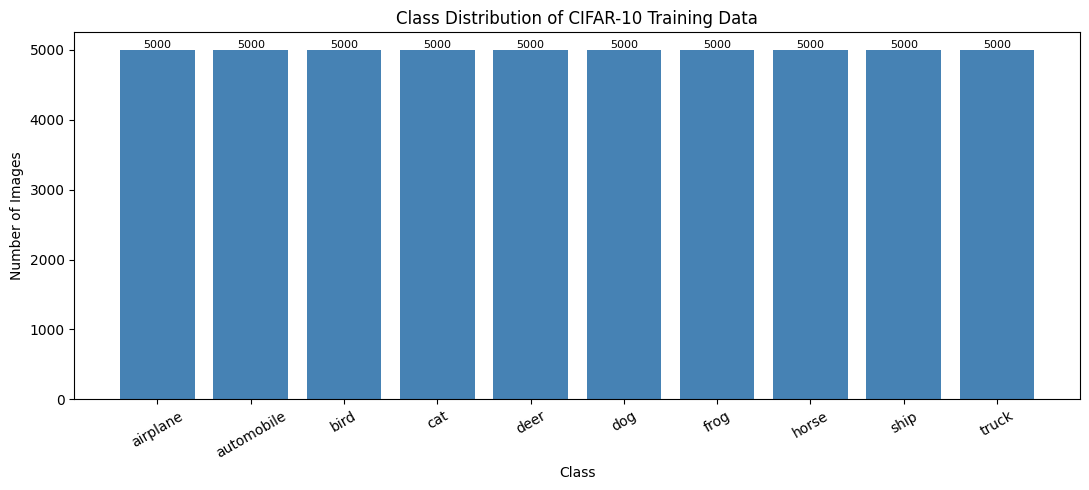
\includegraphics[width=0.85\textwidth]{plot2.png}
\caption{Class Distribution of the CIFAR-10 Training Dataset}
\end{figure}

The bar chart confirms that each of the ten classes contains exactly 5{,}000 training images, indicating a perfectly balanced dataset. This balance ensures that the CNN is not biased towards predicting any particular class more frequently simply because it was over-represented in the training data, so the comparatively weaker performance observed for classes such as cat and dog in Section 11 must be attributed to genuine visual ambiguity rather than class imbalance.

\vspace{0.15cm}

\subsection*{12.3 Feature Maps After Conv1}

\begin{figure}[H]
\centering
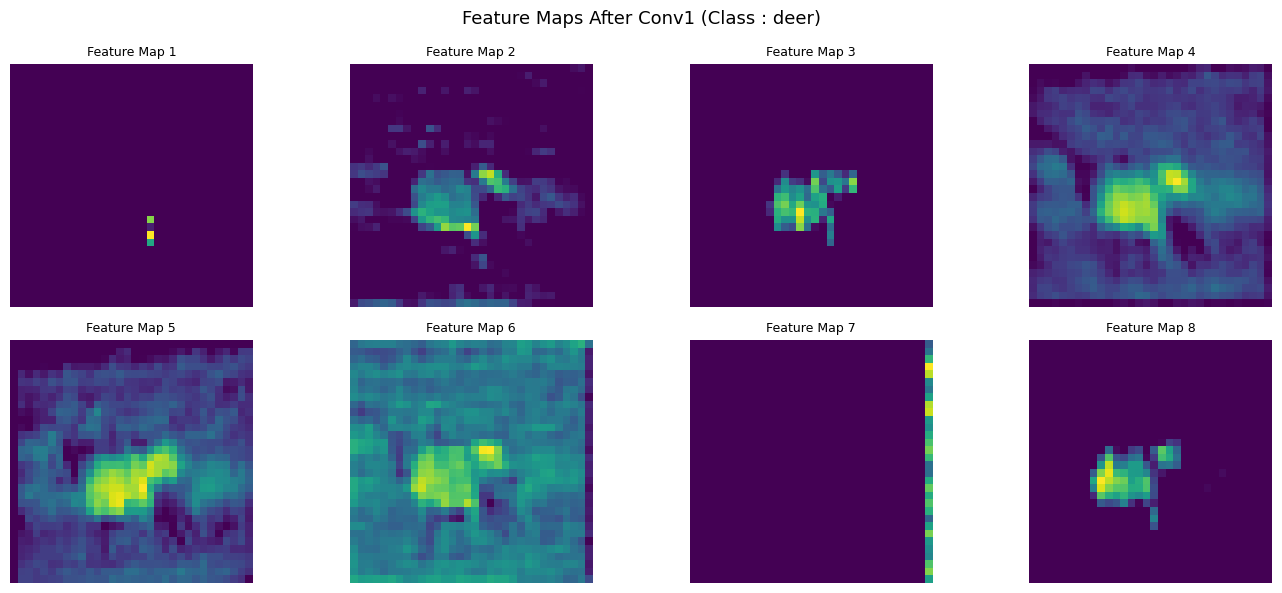
\includegraphics[width=0.95\textwidth]{plot3.png}
\caption{Eight Feature Maps Generated by the First Convolution Layer for a Sample ``Deer'' Image}
\end{figure}

The eight feature maps show that different filters in the first convolution layer respond to markedly different visual patterns present in the same input image. Feature Maps 2, 4, 5, 6 and 8 all show a bright, blob-like region roughly corresponding to the silhouette of the deer's body against the background, indicating that these filters have learned to respond to the animal's overall shape and texture, whereas Feature Maps 1 and 7 remain almost entirely dark except for a thin strip of activation, suggesting these particular filters are tuned to a narrow, specific edge orientation that is largely absent from this image. This diversity of responses across channels, even at the very first convolution layer, is exactly the behaviour expected of a CNN that has begun to learn a varied bank of low-level feature detectors.

\vspace{0.15cm}

\subsection*{12.4 Pooling Comparison}

\begin{figure}[H]
\centering
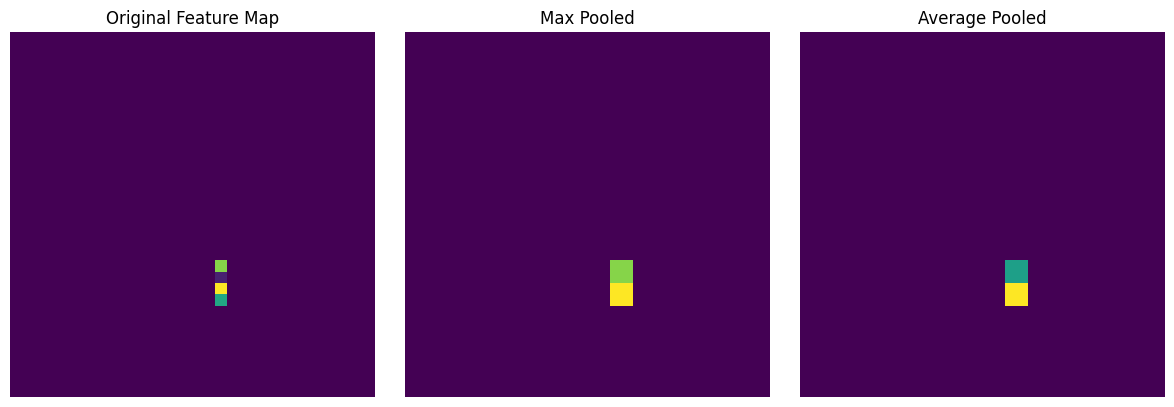
\includegraphics[width=0.95\textwidth]{plot4.png}
\caption{Original Feature Map Compared Against Max-Pooled and Average-Pooled Outputs}
\end{figure}

The original feature map used for this comparison is almost entirely inactive except for a small vertical strip of three high-intensity pixels. The max-pooled output preserves this strip essentially unchanged in colour and position, since the maximum value within each pooling window is retained regardless of its neighbours, whereas the average-pooled output visibly dulls the same pixels, since each pooled value is now an average that includes the surrounding, largely zero-valued activations. This directly illustrates why max pooling is generally preferred when the goal is to retain sharp, localized features such as edges, while average pooling is better suited to producing smoother, more generalized summaries of a feature map.

\vspace{0.15cm}

\subsection*{12.5 Training vs Validation Accuracy}

\begin{figure}[H]
\centering
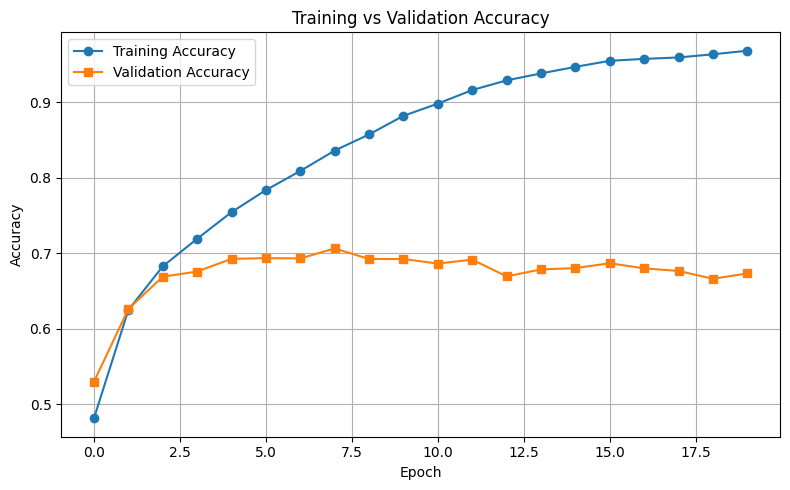
\includegraphics[width=0.75\textwidth]{plot5.png}
\caption{Training and Validation Accuracy vs Epoch}
\end{figure}

The training accuracy curve rises almost monotonically throughout all 20 epochs, ultimately approaching 97\%, while the validation accuracy curve climbs sharply for roughly the first seven epochs before plateauing around 69--71\% and then drifting slightly downward towards 67\% by the final epoch. The widening gap between the two curves from around epoch 8 onward is a textbook signature of overfitting, with the network continuing to memorize training-specific details long after it has stopped generalizing better to unseen validation images.

\vspace{0.15cm}

\subsection*{12.6 Training vs Validation Loss}

\begin{figure}[H]
\centering
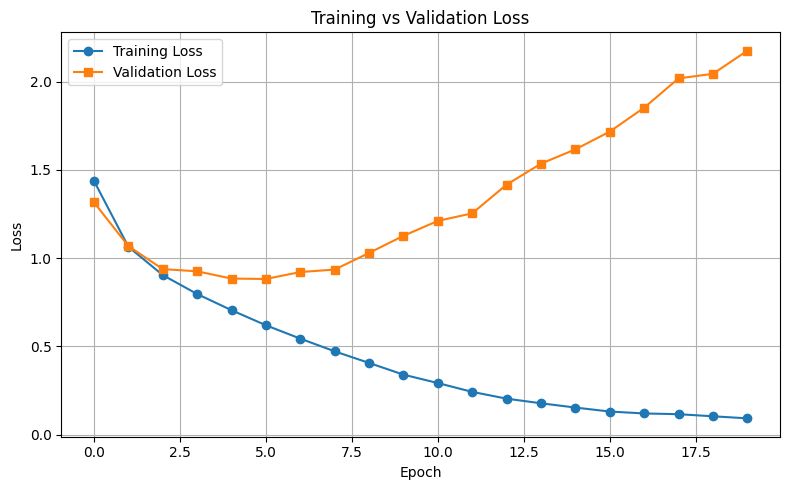
\includegraphics[width=0.75\textwidth]{plot6.png}
\caption{Training and Validation Loss vs Epoch}
\end{figure}

The training loss decreases smoothly and continuously across all 20 epochs, falling from 1.44 to below 0.10, whereas the validation loss falls alongside it only until roughly epoch 5--6, after which it reverses direction and climbs steadily to over 2.1 by epoch 20. This clean divergence between a monotonically falling training loss and a rising validation loss is a stronger and more direct indicator of overfitting than the accuracy curves alone, and it confirms that the second half of training contributed little additional generalization benefit despite the continued reduction in training loss.

\vspace{0.15cm}

\subsection*{12.7 Confusion Matrix}

\begin{figure}[H]
\centering
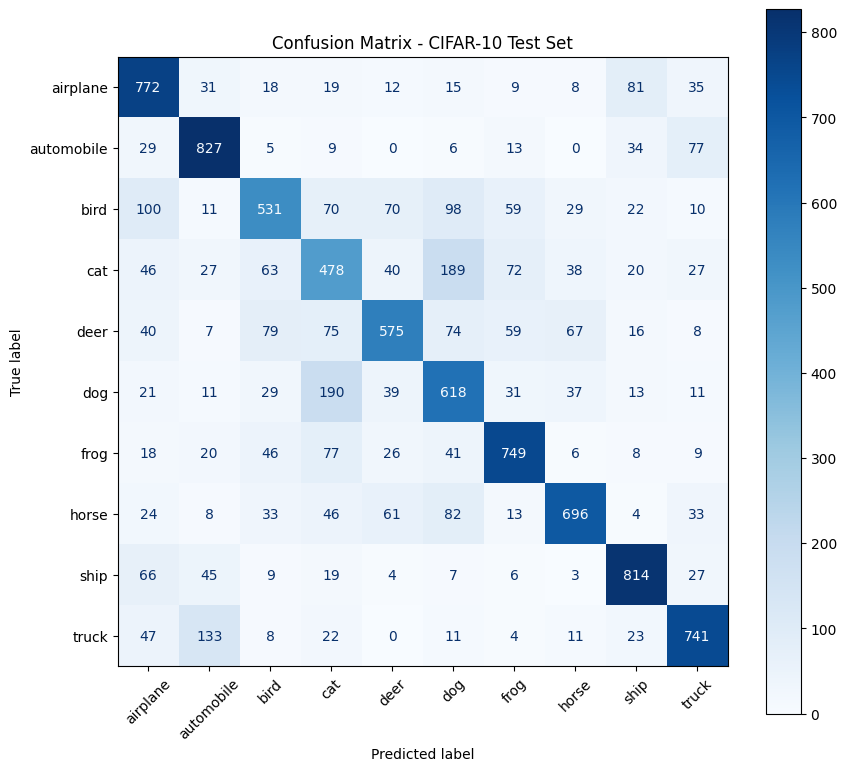
\includegraphics[width=0.8\textwidth]{plot7.png}
\caption{Confusion Matrix of the CNN on the CIFAR-10 Testing Set}
\end{figure}

The confusion matrix shows a strong diagonal, confirming that the majority of test images from every class were classified correctly. The most prominent off-diagonal confusions occur between cat and dog (189 cats predicted as dogs, 190 dogs predicted as cats), consistent with the weak per-class metrics for these two classes noted in Section 11, and between automobile and truck (133 automobiles predicted as trucks), reflecting the visual similarity between these two vehicle categories at low resolution. Vehicle and animal classes are rarely confused with one another (for example, very few airplanes are predicted as cats or dogs), indicating that the network has successfully learned the broad, high-level distinction between animate and inanimate object categories, even where it struggles with finer-grained distinctions within each group.

\section*{13. Results Summary}

\begin{center}
\begin{tabular}{|p{6cm}|p{5cm}|}
\hline
\textbf{Metric} & \textbf{Value}\\
\hline
Training Accuracy & 96.81\%\\
\hline
Testing Accuracy & 68.01\%\\
\hline
Precision & 68.21\%\\
\hline
Recall & 68.01\%\\
\hline
F1-Score & 67.88\%\\
\hline
Number of Parameters & 545{,}098\\
\hline
\end{tabular}
\end{center}

\section*{14. Result Analysis}

The 28.8-percentage-point gap between the final training accuracy (96.81\%) and the final testing accuracy (68.01\%) is the single most important observation of this experiment, and is corroborated by every other piece of evidence gathered: the validation accuracy plateaus and then declines from epoch 8 onward, the validation loss rises continuously from around epoch 6 while the training loss keeps falling, and the network's own first-layer feature maps and pooling behaviour show it is extracting reasonable low-level features, yet the fully connected head, which contains 96\% of the network's 545{,}098 parameters, appears to memorize training-specific detail rather than learning features that generalize equally well to the testing set. Despite this overfitting, a testing accuracy of 68.01\% represents a substantial and expected improvement over both random guessing (10\%) and the kind of MLP baseline studied in Experiment 2, since the two convolution layers allow the network to exploit spatial locality and translation invariance in a way that a purely fully connected architecture, operating on flattened pixels, cannot. The per-class results further show that the network's errors are concentrated almost entirely within semantically related class pairs (cat/dog, automobile/truck) rather than scattered randomly across unrelated categories, indicating that the learned representation, while imperfect, is capturing genuinely meaningful visual structure rather than noise.

\section*{15. Discussion}
 
\subsection*{1. Why is convolution preferred over fully connected layers for images?}
 
A fully connected layer gives every pixel its own weight, ignoring spatial structure and needing huge parameter counts. Convolution instead shares one small kernel across every location, cutting parameters sharply (896 vs 524{,}416 for FC1) while assuming useful features like edges and textures are local and translation-invariant, so the same detector works anywhere in the image.
 
\subsection*{2. How does stride affect the feature map size?}
 
The output size follows $\lfloor(N-F+2P)/S\rfloor+1$, so stride $S$ sits in the denominator: a larger stride skips more positions, visiting fewer locations and shrinking the feature map. Raising stride from 1 to 2 on a $32\times32$ input with a $3\times3$ kernel and no padding reduced the output from $30\times30$ to $15\times15$, roughly halving each dimension.
 
\subsection*{3. What is the role of padding?}
 
Padding adds extra border rows/columns, usually zeros, before convolution. It compensates for edge pixels visited fewer times than interior ones, and lets output size be controlled independently of kernel size. ``Same'' padding chooses $P$ so output matches input resolution, letting deep networks avoid premature shrinkage, while ``Valid'' padding (no padding) always produces a smaller output.
 
\subsection*{4. Why is pooling used?}
 
Pooling summarizes each local window into one value, reducing spatial resolution and the computation and parameters needed downstream, while adding translation invariance since small shifts within a window don't change the pooled result. Max pooling keeps the strongest activation in each window, making it effective at preserving prominent edges and shapes while discarding less informative detail.
 
\subsection*{5. How do feature maps represent image characteristics?}
 
Each feature-map channel is produced by a different learned kernel, so it marks where a particular visual pattern occurs. Several Conv1 channels showed a bright blob tracing the sample deer's silhouette, meaning those filters respond to its shape and texture, while other channels stayed nearly inactive, tuned instead to patterns like specific edges absent from this image.
 
\subsection*{6. Why do CNNs require fewer parameters than MLPs?}
 
CNNs need fewer parameters because a kernel is shared across every spatial position, so parameter count depends only on kernel size and channels, not image size. An MLP needs a unique weight per pixel-neuron connection instead. Here, Conv1 needs just 896 parameters versus 524{,}416 for FC1 -- over 585 times more, despite FC1 taking a smaller, already-pooled input.
 
\section*{16. Additional Exercise Solutions}
 
\subsection*{Exercise 1: Output size for a $64\times64$ image, $5\times5$ kernel, stride 2, padding 2}
 
Using the output-size formula from Section 3 with $N=64$, $F=5$, $P=2$ and $S=2$
 
\[
\left\lfloor\frac{64-5+2(2)}{2}\right\rfloor+1 = \left\lfloor\frac{63}{2}\right\rfloor+1 = 31+1 = 32
\]
 
the resulting feature map has spatial dimensions $32\times32$. This shows that even with a fairly large $5\times5$ kernel, sufficient padding ($P=2$) combined with a stride of 2 keeps the output at exactly half the input resolution rather than shrinking it further, which is a common design choice when a network needs to downsample deliberately while still controlling the exact output size analytically, rather than relying purely on a separate pooling layer. It also illustrates that padding and stride can be tuned together to hit a target output size for a given kernel and input, which is useful when designing deeper architectures.
\newpage
\subsection*{Exercise 2: Trainable parameters of a convolution layer with 64 filters of size $3\times3$ on an RGB input}
 
Using the convolution parameter formula from Section 3 with $F=3$, $C_{in}=3$ and $C_{out}=64$
 
\[
(3\times3\times3+1)\times64 = (27+1)\times64 = 28\times64 = 1{,}792
\]
 
so this layer needs 1{,}792 trainable parameters. This is a useful benchmark against the actual CNN built in this experiment, whose first convolution layer instead uses 32 filters and requires only 896 parameters; scaling that same layer up to 64 filters would exactly double its parameter count to 1{,}792, confirming that the number of filters scales the parameter count linearly, independent of the input's spatial resolution. This linear relationship is what makes it straightforward to trade off representational capacity against computation simply by adjusting the filter count of a single convolution layer.
 
\subsection*{Exercise 3: ReLU vs Sigmoid Activation Functions}
 
ReLU, $f(z)=\max(0,z)$, is cheap to compute, does not saturate for positive inputs, and largely avoids the vanishing-gradient problem, which is why it was used throughout this CNN's hidden layers. Sigmoid, $f(z)=1/(1+e^{-z})$, squashes inputs into $(0,1)$ but saturates strongly at both extremes, so its gradient shrinks toward zero there; stacking many such layers causes gradients reaching early layers to vanish almost entirely during backpropagation. This makes Sigmoid a poor choice for deep hidden layers, though it remains useful at output layers needing a bounded, probability-like value between 0 and 1. In practice, ReLU also trains faster since it involves no exponential computation, unlike Sigmoid.
 
\subsection*{Exercise 4: Replacing Max Pooling with Average Pooling}
 
Sections 9 and 12.4 compare max and average pooling on the same feature map: both shrink $32\times32$ to $16\times16$ identically, but max pooling preserves sharp, high-intensity activations almost unchanged, while average pooling blends them with mostly-inactive neighbours, visibly dulling them. Replacing every max pooling layer in this CNN with average pooling would smooth and attenuate the sharp, edge-like activations currently passed forward unchanged at every stage. Based on this behaviour, that change would likely slightly reduce the network's ability to preserve fine, high-contrast detail such as animal-background boundaries, typically producing a marginally lower accuracy on a texture-sensitive dataset like CIFAR-10, though the gap is usually modest since spatial downsampling stays the same.
 
\subsection*{Exercise 5: Increasing Convolution Filters from 16 to 64}
 
This CNN already uses 32 and 64 filters rather than a 16-filter baseline, and Section 8 shows why filter count matters: since parameters scale as $(F\times F\times C_{in}+1)\times C_{out}$, raising filter count from 16 to 64 multiplies that layer's parameters -- and its multiply-accumulate operations in both forward and backward passes -- by four, directly increasing per-epoch training time. A larger filter bank can learn a richer, more varied set of feature detectors, as seen in Section 12.3's varied feature maps, typically improving accuracy up to a point. However, given the 28.8-point training-testing accuracy gap already observed, simply adding more filters without regularization such as Dropout or Batch Normalization would likely widen overfitting rather than meaningfully improving test accuracy.
 

\section*{17. Conclusion}

A Convolutional Neural Network was implemented in PyTorch and trained on the CIFAR-10 dataset for multi-class image classification, following a systematic sequence of tasks covering the convolution operation, stride and padding, feature map visualization, pooling and full network training and evaluation. The convolution kernel-size and hyperparameter studies confirmed the theoretical output-size relationship $\lfloor(N-F+2P)/S\rfloor+1$ exactly, the programmatically calculated parameter count of 545{,}098 matched PyTorch's own count exactly, and the pooling comparison confirmed the expected qualitative difference between max pooling's sharp feature preservation and average pooling's smoothing behaviour. The final CNN, comprising two convolution-ReLU-MaxPool blocks followed by two Dense layers, was trained for 20 epochs using the Adam optimizer and achieved a final training accuracy of 96.81\% but a considerably lower testing accuracy of 68.01\%, with a weighted precision of 68.21\%, recall of 68.01\% and F1-score of 67.88\%. The training and validation accuracy/loss curves, together with the confusion matrix, consistently identified overfitting -- driven primarily by the 524{,}416-parameter fully connected layer following the flattening operation -- as the dominant limitation of the current model, with the cat and dog classes, and to a lesser extent automobile and truck, contributing disproportionately to the remaining classification errors due to genuine visual similarity between these class pairs. Overall, the experiment reinforced practical understanding of the convolution operation, parameter sharing, pooling strategies, and CNN training and evaluation using standard classification metrics, and highlighted regularization (such as Dropout, weight decay or data augmentation) as the most promising direction for improving generalization in future iterations of this architecture.

\section*{18. References}

\begin{enumerate}

\item Ian Goodfellow,
Yoshua Bengio,
Aaron Courville,
\textit{Deep Learning},
MIT Press,
2016.

\item Christopher M. Bishop,
\textit{Pattern Recognition and Machine Learning},
Springer,
2006.

\item Simon Haykin,
\textit{Neural Networks and Learning Machines},
Pearson Education,
2009.

\item Alex Krizhevsky,
\textit{Learning Multiple Layers of Features from Tiny Images},
Technical Report, University of Toronto,
2009.

\url{https://www.cs.toronto.edu/~kriz/cifar.html}

\item PyTorch Documentation.

\url{https://pytorch.org/docs/stable/index.html}

\item TorchVision Datasets Documentation.

\url{https://pytorch.org/vision/stable/datasets.html}

\item Scikit-learn Documentation.

\url{https://scikit-learn.org}

\end{enumerate}

\section*{19.Source Code}

The complete implementation was carried out in Python using Google Colab.
\\[10pt]
\url{https://github.com/K-Mithran/Deep-Learning/blob/main/Lab3/DL_3.ipynb}
\\[10pt]

\vfill

\end{document}
